% EGOS paper
% Version 1.0 January 2009
%

\documentclass[a4paper, 12pt]{article}

% Use arial
\usepackage{helvet}
\renewcommand{\familydefault}{\sfdefault}

% Use Times New Roman
%\usepackage[T1]{fontenc}
\usepackage[utf8]{inputenc}
\usepackage{mathptmx}

% drozas: Added for customization
\usepackage[hyphens]{url}
\usepackage{titling}
\setlength{\droptitle}{-2.7cm}


\usepackage[style=apa, backend=biber, urldate=long]{biblatex}
\DeclareLanguageMapping{british}{british-apa}
\addbibresource{egos2015_full_paper_drupal_at.bib}
\usepackage[british]{babel}
\usepackage{csquotes}
\usepackage{setspace}
\usepackage[top=3.2cm, left=2.5cm, right=2.5cm, bottom=4.3cm]{geometry}
\setlength{\footskip}{3cm}

\usepackage[utf8]{inputenc}

\usepackage{titlesec}
\setcounter{secnumdepth}{4}
\titleformat{\paragraph}
{\normalfont\normalsize\bfseries}{\theparagraph}{1em}{}
\titlespacing*{\paragraph}
{0pt}{3.25ex plus 1ex minus .2ex}{1.5ex plus .2ex}

%% Paragraph settings
\setlength{\parskip}{0.9em}

% drozas: Urls
\usepackage{hyperref}

% drozas: Ordinals and numbering
\usepackage[super]{nth}
\usepackage[gen]{eurosym}

% amsmath package, useful for mathematical formulas
\usepackage{amsmath}
% amssymb package, useful for mathematical symbols
\usepackage{amssymb}

% graphicx package, useful for including eps and pdf graphics
% include graphics with the command \includegraphics
\usepackage{graphicx}

% cite package, to clean up citations in the main text. Do not remove.
%\usepackage{cite}

\usepackage{color} 

% Use doublespacing - comment out for single spacing
%\usepackage{setspace} 
\onehalfspacing

\usepackage{authblk}
\renewcommand\Affilfont{\itshape\small}

% Text layout
%\topmargin 0.0cm
%\oddsidemargin 2.5cm
%\evensidemargin 2.5cm
%\textwidth 16cm 
%\textheight 21cm

% Bold the 'Figure #' in the caption and separate it with a period
% Captions will be left justified
\usepackage[labelfont=bf,labelsep=period,justification=raggedright]{caption}

% Use the PLoS provided bibtex style
%\bibliographystyle{plos2009}

% Remove brackets from numbering in List of References
%\makeatletter
%\renewcommand{\@biblabel}[1]{\quad#1.}
%\makeatother

\usepackage{titling}
\newcommand{\subtitle}[1]{%
  \posttitle{%
    \par\end{center}
    \begin{center}\large#1\end{center}
    \vskip0.5em}%
}

% Leave date blank
\date{}

\hyphenation{ac-ti-vi-ties}
\begin{document}


\title{Drupal as a runaway object: conceptualisation of peer production activities through Activity Theory}
\subtitle{Sub-theme 17: ``Activity Theory and Organizations''}
\author[1]{David Rozas\thanks{drozas@surrey.ac.uk}}
\author[1]{Nigel Gilbert\thanks{n.gilbert@surrey.ac.uk}}
\author[1]{Paul Hodkinson\thanks{p.hodkinson@surrey.ac.uk}}
\affil[1]{Department of Sociology, University of Surrey, Guildford, United Kingdom}
\maketitle

%\begin{center}
%{\large Sub-theme 17: ``Activity Theory and Organizations''}
%\end{center}


\section*{Abstract}

The lack of clear boundaries and the distributed nature of Commons-Based Peer Production (CBPP) pose a challenge for the theoretical frameworks which aim to provide a useful methodological tool for its conceptualisation and analysis, such as Activity Theory (AT).
This paper presents the use of AT in the ongoing study of the organisational dynamics of a large and diverse CBPP community: Drupal. This application of AT is being carried out by drawing on the model of activity system to analyse contribution activities; and by conceptualising Drupal as a runaway object, which operates as a nexus for the study of these coordination efforts.
Hence, by presenting the conceptualisation and challenges which are currently being faced, this paper aims to provide evidence of the value of AT to untangle the dense and multidirectional dynamics which lie within these communities, as well as to contribute to the discussion on the limitations that this approach could have for the study of peer production.


Keywords: Activity Theory, case study, Commons-Based Peer Production, Drupal, Free/Libre Open Source Software, Science \& Technology Studies

\newpage
\section{Introduction}

The term Commons-Based Peer Production (CBPP) was originally coined by \textcite{Benkler2002} to define a new model of socio-economic production in which groups of individuals cooperate with each other to produce meaningful products without a traditional hierarchical organisation \parencite{benkler2006wealth}. It is characterised as not being primarily driven by private appropriation and as favouring reproducibility and derivativeness \parencite[11-12]{Fuster2014}. For example, in the case of digital commons, this results in the openness of the outcomes and processes.

CBPP is spreading to very diverse areas of activity, from open science to urban commons \parencite[121-124]{Fuster2014}. Nevertheless, Free/Libre Open Source Software (FLOSS) represents the pioneering and most developed area of CBPP \parencite[121]{Fuster2014}. FLOSS is software which allows its use, copy, study and modification in any way. These rights are protected by certain licences, such as the GNU General Public License, on the source code: the set of computer instructions written in a programming language which compose a specific FLOSS.

The invention of the World Wide Web in 1989 \parencite{berners1992world} and its spread during the following years created new possibilities of collaborative production, including the collaborative development of software. FLOSS communities quickly benefited from these new possibilities by experimenting with these innovative ways of collaboration and development models \parencite{kelty2008two-linux}. The growth of FLOSS in the forthcoming years was enormous. For example, the study by \textcite{deshpande2008total} of more than 5,000 active and popular FLOSS projects during the period 1995-2006 concluded that the number of code additions, the total size of the projects in lines of code and the number of projects grew exponentially.

Hence, FLOSS provides a cutting-edge area for the study of the organisational and structurational dynamics of large CBPP communities that produce and maintain these commons. However, the distributed nature and lack of clear boundaries of these groups present a challenge not only for its study, but also for the theoretical frameworks which aim to provide a useful methodological tool for its conceptualisation and analysis, such as Activity Theory (AT).

\textcite{engestrom2007communities} initiated a discussion about the challenges that peer production poses for the model of activity system, due to the characteristics of CBPP communities. Drawing on the mycorrhizae metaphor, \textcite[10-11]{engestrom2007communities} provided an account of the characteristics of these communities, as being ``difficult if not impossible to bound and close" and defining their formation as being in a constant living and expanding process. In a subsequent publication \parencite{engestrom_future_2009}, he provided a more concrete description of the concept of benign runaway objects. Citing as examples Wikipedia, organic farming and open research and publishing, he presented a more accurate set of prerequisites for them:

\begin{itemize}
	\item They must have intrinsic properties that transcend the utilitarian profit motive.
	\item The object must yield useful intermediate products, yet remain an incomplete project.
	\item The object must be visible, accessible and cumulable.
	\item There must be effective feedback from and exchange among the participants acting on the object.
\end{itemize}

The ongoing study presented in the following sections of this paper draws on Engeström's concept of runaway object and the model of activity system to improve our understanding of the organisational dynamics in large and diverse CBPP communities. Concretely, this research focusses on Drupal as a case study. Section \ref{sec:drupal} introduces the conceptualisation of Drupal as a runaway object. Sections \ref{subsec:modules-concept} and \ref{subsec:dcamp-concept} provide examples of its application to the study of two different peer production activities: the development of source code  and the organisation of Face-to-face (F2F) events. Section \ref{sec:discussion-future} provides a discussion of the value of AT to lead the emergence, through data, of the questions and dimensions to be explored in future stages in order to improve our understanding of CBPP. Finally, section \ref{sec:conclusion} concludes the paper describing how the model of activity system is proving to be of value in the study of peer production.


\section{Drupal as a runaway object and the exploration of self-organisation via contribution activities}
\label{sec:drupal}

This ongoing study focusses on the Drupal community with the aim of improving our understanding of organisational dynamics in large and diverse CBPP communities. Drupal is a FLOSS content management framework released in 2001 \parencite{drupal-history:2013:Online} which provides a robust platform for the development of web applications. It currently powers 2\% of the websites worldwide \parencite{cms-usage:2013:Online}. 
This percentage includes enormously popular websites with complex architectures and high loads of traffic, such as whitehouse.gov, mtv.co.uk or economist.com, among others. Drupal represents one of the most vibrant examples of the success of FLOSS. For example, in the latest annual ``Future of Open Source Survey" based on 1,240 responses, Drupal was the third most valued FLOSS project \parencite{future-open-source-survey:2015}.

The Drupal community has been growing constantly: there are currently more than 1 million people registered at the main platform of collaboration (Drupal.org), and more than 30,000 committers of source code \parencite{drupal-about:2013:Online}. The community is also highly active offline, with thousands of events of different scope (local, regional, national and international) being held all around the World every year \parencite{DrupalEvents2010}.

This ongoing study of Drupal as a CBPP community develops from the concept of a benign runaway object as defined by \textcite{engestrom_future_2009}. As any other FLOSS, Drupal transcends the utilitarian motives and bases its sustainability on collaborative production. The nature of the project is dynamic, it is in a constant process of change. In addition, the main production processes and project outcomes are also visible and accessible all of the time. Figure \ref{drupal_runaway_object} provides a graphical description of this approach, in which the structures are not so well defined and are subsumed by the object.


\begin{figure}[h]
	\centering
	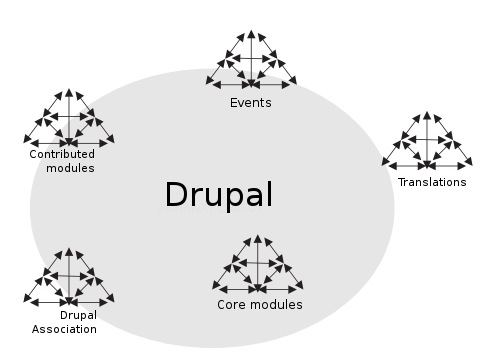
\includegraphics[scale=0.6]{img/drupal_runaway_object.png}
	\caption[Conceptualisation of Drupal as a runaway object]%
	{Conceptualisation of Drupal as a runaway object. Based on figure 19.2 of \textcite{engestrom_future_2009}.}
	\label{drupal_runaway_object}
\end{figure}

The concept of a runaway object successfully captures the challenges which are being faced for the conceptualisation of this case study. As identified by \textcite[305]{engestrom_future_2009}, in peer production the ``object is pervasive and its boundaries hard to draw". This provokes ambiguity in the position of these activity systems, being ``subsumed by the object rather than in control of it" \parencite[305]{engestrom_future_2009}.

Nevertheless, although in peer production the ``boundaries and structures of activities systems seem to fade away" \parencite[309]{engestrom_future_2009}, this mode of production requires and creates ``bounded hubs of concentrated coordination efforts" \parencite[310]{engestrom_future_2009}. In this way, the application of the model of activity system for the analysis of these hubs of effort remains very valuable.
As argued by \textcite{Uden2007}, the use of the activity system as a unit of analysis incorporates notions such as social rules, mediating artefacts or division of labour, as part of a dynamic phenomenon, avoiding simple causal explanations in the study of FLOSS. This ongoing study is exploring some of these bounded hubs in order to shed light on how a large and diverse CBPP community such as Drupal organises itself, concretely, by exploring some of the contribution activities in the case study. Hence, the concept of a runaway object operates as a nexus for these contribution activities.

Focussing on contribution activities using AT as a lens will offer the possibility to explore the relationships between the artefacts employed for the collaboration, the roles played by its members (division of labour) and the implicit and explicit rules, among others, with respect to the development of Drupal as a runaway object. Additionally, AT offers the advantage of performing historical analyses of the community behind it, allowing a contextual study of the local practices and the emerging structures in it \parencite{Uden2007}.

With that objective in mind, an identification of which activities are understood as contributions by members of the Drupal community was carried out during the first phase of this study \parencite{rozas2015}.
This stage followed an ethnographic approach (combining participant observation, semi-structured interviews and documentary analysis), and focussed on identifying activities perceived as contributions through the negotiation processes of members participating in this community.

The next subsections discuss the preliminary conceptualisation through AT of some of the contribution activities which will be explored in depth during subsequent phases of this ongoing study. They are selected to illustrate how the continuing application of AT is helping to lead, through data, the emergence of questions which will improve our understanding of CBPP in future stages, which are described in greater detail in section \ref{sec:discussion-future}.

\subsection{Conceptualising the development of Drupal modules through AT}
\label{subsec:modules-concept}

Drupal modules are sets of source code files that provide certain functionalities in a website running Drupal. A Drupal site can have three different types of modules\footnote{``Module developer's guide'' accessed on \nth{15} December 2014, from \url{https://www.drupal.org/project/drupal}}:

\begin{itemize}
	\item \textit{Core}: modules that are included in the default download of Drupal, and can be seen as its kernel. The core is composed of dozens of modules\footnote{Version 7.34 of Drupal accessed on \nth{22} November 2014, from \url{https://www.drupal.org/project/drupal}, has 41 modules at \texttt{/modules}.}, which are approved by the core developers and the community. 
	\item \textit{Contributed}: modules written by the Drupal community and shared under the same GNU Public License as Drupal in the main platform of collaboration. They provide new functionalities that are not part of the core, and can be seen as ``plugins''. This ecosystem is composed of thousands of modules\footnote{A dynamic directory in the main platform of collaboration accessed on \nth{30} November 2014, from \url{https://www.drupal.org/project/project_module/index?project-status=full&drupal_core=103}, lists 9,769 modules as ``full projects'' (already approved).}.
	\item \textit{Custom}: modules often created for a particular use-case specific to the site.
\end{itemize}

For the proposed example the focus will be placed on the development of contributed modules, whose publication by new developers in the official site requires a peer-reviewing process of the proposed code by other members. In this example, the elements of the activity could be defined as follows \parencite{rozas2014}:

\begin{itemize}
	\item \textit{Subject(s)}: the developer(s) responsible for the development and maintenance of the contributed module (maintainers).
	\item \textit{Instruments, mediating artefacts}: the coordination tools employed by the maintainers and the rest of the members of the community. A typical example of an instrument would be the issues list associated with each module project page. They provide a way of interacting between the maintainers and the rest of the members of the community in which bugs can be reported, new functionalities can be requested and patches\footnote{A patch is a file containing a list of differences in the source code between one set of files and another. The changes in the source code of Drupal are typically done through the submission and application of patches \parencite{drupal-patches:2015:Online}.} can be submitted. It works also as a coordination tool for maintainers themselves. For instance, technical discussions about the different ways of implementing a functionality are often carried out using this artefact. Other types of instruments are IRC\footnote{IRC (Internet Relay Chat) is a protocol which allows real time communication.} channels, direct messages between members of the community (via Drupal.org, e-mail or social networks such as Twitter), Drupal discussion groups\footnote{\url{https://groups.drupal.org/}, accessed on \nth{13} January 2014.} or instruments employed during discussions in offline Drupal events.
	\item \textit{Object}: the contributed module developed as a result of the activity.
	\item \textit{Rules}: the explicit and implicit rules which regulate the development of the module. Examples of explicit rules are the coding standards agreed by the community for the modules\footnote{\url{https://drupal.org/coding-standards}, accessed on \nth{13} January 2014.} or the guidelines for contribution\footnote{\url{https://drupal.org/contribute/development}, accessed on \nth{13} January 2014.}. Examples of implicit rules that could be analysed are those employed by maintainers for the evaluation of the patches submitted by other members without \textit{commit permissions}\footnote{\textit{Commit permissions} refers to the possibility to perform changes in the source code which become part of the official repository, which is hosted in the main platform of collaboration.} on this module. Another example consists of those employed for the estimation of the reputation of contributors who would like to become maintainers of the project. For example, those based on the activity reflected in their user profiles. 
	\item \textit{Community}: all the members of the Drupal community. The interaction with a module is typically due to the fact that they are users of it. They can make use of the instruments to provide feedback about the module, submit patches to solve bugs or extend its functionalities, or provide support related to that module. 
	\item \textit{Division of labour}: this represents the distribution of tasks for the development of the module. An example of a form of division of labour is the allocation of tasks of development according to the different skills of the maintainers. For example, back-end developers, themers or user experience experts, among others. The use of the issues list to allocate tasks between maintainers can be seen as a relationship between the division of labour and the instruments.
\end{itemize}

Figure \ref{drupal_module_at} summarises the relationships between all the entities using the triangular model of activity system of the second generation of AT.

\begin{figure}[h]
	\centering
	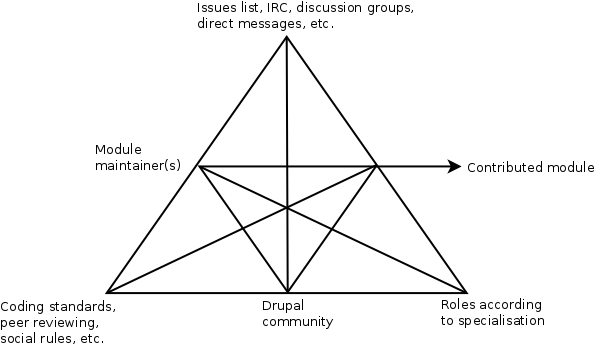
\includegraphics[scale=0.5]{diagrams/drupal_module_at.png}
	\caption{Conceptualisation of the development of contributed modules from an AT perspective.}
	\label{drupal_module_at}
\end{figure}

Regarding the analysis and discovery of conflicts in the system, AT offers a powerful tool for the exploration of tensions. As an illustration, the tensions between the designers and the developers found by \textcite{Zilouchian2011} in their study on consensus building in Drupal, might be analysed using AT as a theoretical lens. In this case, AT provides a useful framework to explore the relationships between the division of labour as a source of tension with respect to the rest of the elements.

This example focusses on the development of contributed modules as a peer production activity. However, a similar approach will be taken for core modules. It will consist of an exploration of the interactions between the different elements, outcomes, connections and tensions between these activities and others. For example, what are the differences in the dynamics and social practices between the collaboration processes of contributed modules with respect to core modules?

The third generation of AT will be applied as well for the study of the tensions between contribution activities. For example, there are tensions arising from the decisions relating to which modules are to be included as core in a major release of Drupal. These tensions can be studied by drawing on the concept of shared objects between two or more activity systems of the third generation of AT \parencite{engestrom_future_2009}. Figure \ref{drupal_core_contrib} depicts a preliminary conceptualisation of potentially shared objects (modules' source code) in this case study. 

\begin{figure}[h]
	\centering
	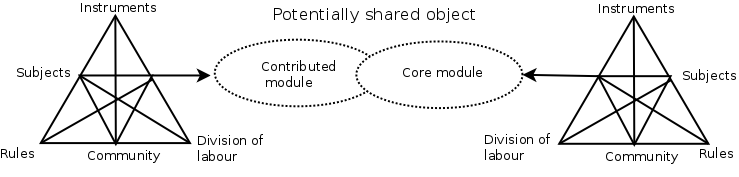
\includegraphics[scale=0.44]{diagrams/drupal_core_contrib.png}
	\caption[Conceptualisation of Drupal as a runaway object]%
	{Illustration of two activity systems and a potentially shared object in the Drupal community. Based on figure 19.1 of \textcite{engestrom_future_2009}.}
	\label{drupal_core_contrib}
\end{figure}



\subsection{Conceptualising the organisation of Face-to-face events as contribution activities from an AT perspective}
\label{subsec:dcamp-concept}

One of the key findings from the initial stage of this ongoing study is the relevance of F2F events in the Drupal community, as well as the way several activities related to them are perceived as contributions by its members \parencite{rozas2015}. It exposes the need to broaden our understanding of contribution activities in FLOSS communities. Although less visible, these activities foster collaboration by creating or modifying the emotional experiences of their participants. 

These events differ significantly in scope, target audience and size. For example, local events typically have dozens of participants. They vary from the most informal and social (e.g. Drupal Beer and Chat), to events focussed on presentations about case studies or the technical advancements of the platform with learning purposes (e.g. Drupal Show and Tell). On the other hand, larger events such as DrupalCamps have hundreds of participants, and have a regional or national scope. The organisation of these is carried out by the local communities, but some of the processes of participation are more formalised than in local events. For example, the processes of submission of presentations are peer-reviewed in a similar way to those in academia. Finally, DrupalCons are international events intended for a broader audience. They have thousands of participants, and many of the organisational activities are largely managed by the most formal institution within the Drupal community: the Drupal Association.

This ongoing study aims to explore the different dynamics, outcomes and organisational processes that surround these events. 
A preliminary conceptualisation of the contribution activity ``participation in a DrupalCamp'' is depicted in figure \ref{drupalcamp_at}, including the following elements:

\begin{itemize}
	\item \textit{Subject(s)}: the participant(s) in the event.
	\item \textit{Instruments, mediating artefacts}: the coordination tools employed by the organisers and the rest of the members of the community. For example, the main website developed for the event, mailing lists or specific groups at Drupal.org.	
	\item \textit{Object}: the DrupalCamp event.
	\item \textit{Rules}: the explicit and implicit rules which surround the event. Examples of explicit rules are the selection criteria for the presentations\footnote{See \url{http://2012.drupalcamp.es/en/node/23.html} (accessed on \nth{19} May 2015) for an example of speaker guidelines, in this case the ones used at DrupalCamp Spain 2012.}, or codes of conduct\footnote{See \url{http://www.drupalcampbrighton.co.uk/content/code-conduct} (accessed on \nth{19} May 2015) for an example of a code of conduct, in this case the one used at DrupalCamp Brigthon 2015.} outlining the shared ideals and values of the community. An example of implicit rules is social rules related to the reputation of a subject in the community.
	\item \textit{Community}: all the members of the Drupal community.
	\item \textit{Division of labour}: the different roles of the participants during the event, for example, session reviewers, attendees or presenters.
\end{itemize}


\begin{figure}[h]
	\centering
	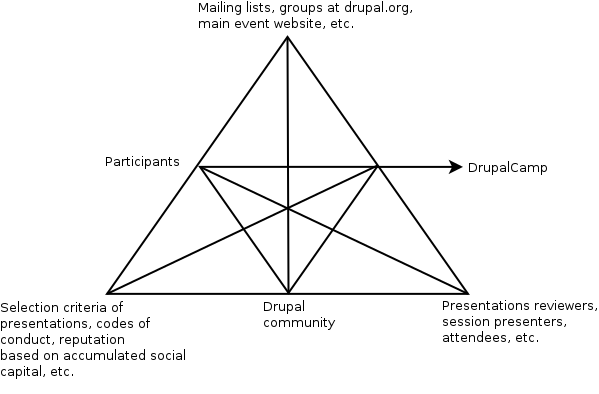
\includegraphics[scale=0.65]{diagrams/drupalcamp_at.png}
	\caption{Conceptualisation of the participation in a DrupalCamp from an AT perspective.}
	\label{drupalcamp_at}
\end{figure}

Using AT as a lens for the study of these peer production activities will facilitate the analysis of its dynamics, its outcomes and the exploration of the relationships between the different elements. This approach will be similar to that intended for the study of the development of core and contributed modules (section \ref{subsec:modules-concept}). 

Equally, the notion of tensions can also be incorporated, for example, to analyse the tensions related to having more horizontal and transparent procedures with regard to the selection of the presentations. Using AT as a lens, these tensions could be framed by exploring their impact on the entities. For example, their impact on the rules, leading to the creation of explicit guidelines; or their impact in the artefacts, provoking the inclusion of peer-reviewing systems in the website of the event to improve the transparency of the process.


\section{Discussion and future work}
\label{sec:discussion-future}

The lack of clear boundaries and the distributed nature of peer production represents a challenge for the model of activity system as a unit of analysis \parencite{engestrom_future_2009}. The case presented in this paper aims to provide evidence of the value of AT as a methodological tool for the study of peer production. 

Firstly, the use of the model of activity as a unit of analysis helped in reconsidering the notion of contribution activities in these communities, leading to the emergence of certain contribution activities which remain less visible in these communities \parencite{rozas2015}. Secondly, AT provides a flexible framework to analyse the organisational dynamics, the relationships between entities, its tensions and its outcomes, from significantly diverse but relevant contribution activities. In this way, the conceptualisation of Drupal as a runaway object operates as a nexus for them. Thus, it facilitates the conceptualisation of Drupal as being shared by all these contribution activities, despite the diversity of the subjects carrying them out, the multi-faceted nature of its medium and the intermittent nature of these hubs of collaboration.

Studying the organisational processes of some of these contribution activities with the aid of AT as a lens, as described in section \ref{sec:drupal}, will allow the main objective to be explored: to improve our understanding of how large and diverse CBPP communities organise themselves.

In addition, the use of the contribution activity as a unit of analysis led to the emergence of the dimensions employed for the sampling in the next stage of this study: its online\slash offline dimension and its degree of formalisation.

The online\slash offline dimension can be understood as a blurred and continuous one. ``Mostly online" contribution activities are those in which actions and operations, from an AT perspective, are mostly performed in the online medium. For instance, in the development of source code for core or contributed modules, most actions and operations are typically carried out online. However, offline events, such as Drupal \textit{hackathons} \parencite{lapp20072006}, are interconnected with this type of contribution activity, and also play a relevant role. In a similar way, the impact of online artefacts, such as the use of online platforms including peer-reviewing mechanisms, to the organisational dynamics of F2F events represents an example of the multi-faceted nature of this dimension in the other direction.

Regarding the level of formalisation, significantly different dynamics are being observed in contribution activities with respect to this dimension for both ``mostly online" and ``mostly offline" activities.  For example, in the ``mostly online" dimension, the organisational procedures of core with respect to contributed modules are remarkably more formal. This can be noticed, for instance, in the accessibility to perform changes in the source code or the social norms behind the organisation for the development of the modules. A similar insight emerged in the ``mostly offline" dimension, in which significant differences in the dynamics are being observed, depending on the scope of the events. For example, while local and regional events present a higher ``grassroots" set of dynamics in terms of organisational procedures, DrupalCons are more centralised and are becoming institutionalised via the Drupal Association. This effect might resemble what \textcite{shaw2014laboratories} identified in a recent paper as an extension of the Iron law of oligarchy of \textcite{michels1915political} in CBPP communities, becoming more oligarchic as they grow. A preliminary sampling of the contribution activities which will be explored in detail in future stages in order to explore these dynamics based on the emergent categories previously describe is depicted in figure \ref{future-work-activities}. 


\begin{figure}[h]
	\centering
	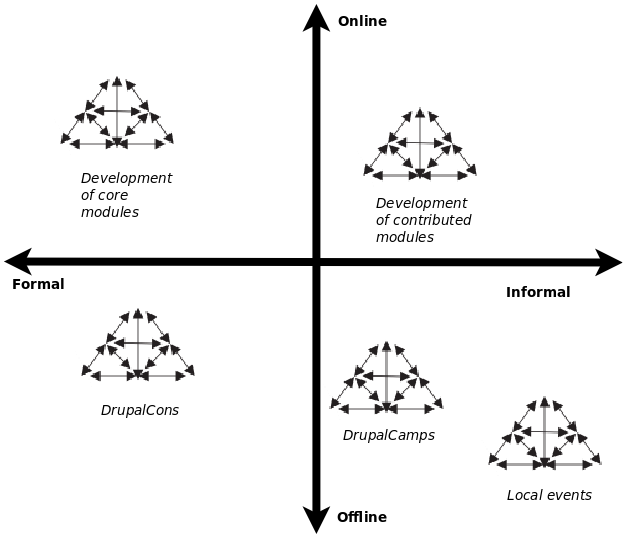
\includegraphics[scale=0.4]{./diagrams/future_work_activities_dimension.png}
	\caption{Diagram summarising the sampling of contribution activities which will be explored in future stages.}
	\label{future-work-activities}
\end{figure}

Hence, the model of activity system provides an appropriate tool for the analysis of CBPP of this case study, in which the boundaries are harder to define than in more traditional modes of production. For example, it provides flexibility for the study of activities as the ones presented, in which the online/offline dimension is blurred, and continuous rather than binary. 


Since this is an ongoing study, the application is still preliminary and limited, and new conceptualisation challenges are expected to be faced during the forthcoming phases. Nevertheless, the preliminary conceptualisation exposed for this case study aims to illustrate how this theoretical framework remains useful for the study of peer production activities.

\newpage
\section{Conclusion}
\label{sec:conclusion}

The study of peer production represents a challenge for theoretical frameworks which aim to provide methodological tools for its conceptualisation and analysis, such as AT. Nevertheless, thanks to its integration with novel concepts such as the one of runaway object, these analytical tools provide value to untangle the dense and multidirectional dynamics which lie within these communities.

In this paper, we aim to show how its application to the study of a large and diverse CBPP, such as Drupal, is proving to be valuable to lead the emergence of questions through data collected following an ethnographic approach. Firstly, by drawing on the model of activity system as a unit of analysis to explore contribution activities. This approach provides a powerful theoretical lens to shed light on the organisational processes of the presented case study. Secondly, by employing the concept of runaway object to conceptualise Drupal as a nexus for these contribution activities, while capturing its pervasiveness and the ambiguity in the positions of its activity systems.

Hence, by presenting the conceptualisation and challenges which are currently being faced in this ongoing study, we aim to contribute to the discussion on the limitations that this approach could have for the study of peer production.

\section*{Acknowledgments}

We thank Sara Lara Márquez (Cass Business School, at the City University London) for her valuable feedback and her encouragement to write this paper. This work was partially supported by the Framework programme FP7 ICT-2013-10 of the European Commission through project \href{http://www.p2pvalue.eu/}{P2Pvalue} (grant no.: 610961).


\printbibliography


\end{document}
